%% ============================================================
%%  Chapter 5 — Data-Driven Temporal Computing with
%%              Polymer-Electrolyte Memristor Reservoirs
%%
%%  NOTE: bound as Chapter 5. Internal labels use the ch5_ prefix and
%%  figures live in figures/chapter5/, matching the bound order.
%%
%%  Author : Carlos David Prado-Socorro
%%  Date   : June 2026
%%  Institution : ICMol, Universitat de València
%%
%%  Compile with: latexmk -pdf  (standalone) or via thesis.tex
%%  Plan + evidence: handouts/12_chapter4_demonstration_plan_v4.md,
%%                   handouts/05_chapter4_data_pipeline.md,
%%                   handouts/04_chapter4_temporal_computing_plan.md
%%  Figures: scripts/ch5_figures.py, scripts/ch5_physio_context.py
%% ============================================================

%% ---- Standalone preamble (skipped when \include'd from thesis.tex) ----
\ifdefined\thesismode\else
  \documentclass[12pt, twoside]{report}
  \usepackage{thesis-format}
  \addbibresource{../bibliography/references.bib}
  \begin{document}
  \setcounter{chapter}{4}     % This is Chapter 5 when built standalone
\fi

%% --- Shared macros (\providecommand: harmless if an earlier chapter declared them) ---
\providecommand{\SY}{\textit{Super Yellow}}
\providecommand{\PEO}{PEO}
\providecommand{\LiTf}{LiOTf}
\providecommand{\NaTf}{NaOTf}
\providecommand{\KTf}{KOTf}
\providecommand{\twoterminal}{two-terminal}
\providecommand{\WESAD}{\textsc{wesad}}
\providecommand{\NARMA}{NARMA-10}
%% Standalone-safe reference into this chapter's Supporting Information
%% (Appendix D). Resolves with \cref in the full thesis; prints a literal
%% label in standalone builds, where the appendix is not included.
\providecommand{\siTempRef}[1]{\ifdefined\thesismode\cref{#1}\else Appendix~D\fi}

%% ============================================================
\chapter{Data-Driven Temporal Computing with Polymer-Electrolyte Memristor Reservoirs}\label{ch:temporal}
%% ============================================================

%% ------------------------------------------------------------
\section{Introduction and Scope}\label{sec:ch5_intro}
%% ------------------------------------------------------------

\Cref{ch:poc,ch:comparative} treated the slow, volatile response of these polymer-electrolyte composites first as a phenomenon to be demonstrated and then as a property to be controlled. This chapter treats it as a computational resource. The guiding idea is simple: a device whose conductance carries a fading record of its recent input is, in miniature, a temporal processor, and a collection of such devices is a \emph{reservoir} --- a physical substrate that projects a time-varying input into a high-dimensional state from which simple, linear read-outs can solve temporal tasks.

The chapter rests on a single thesis that connects it to \cref{ch:comparative}: composition and drive \emph{set} the device timescale, and a task \emph{selects} the timescale it needs. The design problem is therefore one of \emph{matching}, and the open question is what a \emph{spread} of timescales --- the low-cost, intrinsic heterogeneity of a solution-processed device family --- buys on top of a single well-chosen one. The destination is a concrete application: low-power, wearable \emph{affective computing} --- the machine recognition of human emotional and physiological state --- whose signals are slow, multi-timescale, and a natural match to these devices. The evidence moves from task-agnostic reservoir benchmarks, to real physiological streams, to \WESAD{} affective classification, and finally to deployment-style tests under sensor noise, consumer wrist-band sensing, and energy and training-cost constraints.

The evidence base is intentionally constrained. Every result is \emph{in silico}: each device node is a compact behavioural model whose parameters are taken directly from the \cref{ch:comparative} fits (\cref{sec:ch5_model}), and every read-out is a single linear regression, so that no claimed computation can be hidden in a nonlinear decoder or a hand-tuned dynamical system. No new devices are fabricated. Two demonstrations run throughout: Demonstration~A asks whether a \emph{single} composition suffices for a single-timescale feature, and Demonstration~B asks what a heterogeneous \emph{bank} adds when the target is multi-timescale. The scoped answer is that the measured device models support temporal-computing demonstrations under constrained read-out conditions, that fading memory is the active ingredient, and that timescale heterogeneity is valuable for memory breadth and task generality but not a guaranteed improvement on every task.

%% ------------------------------------------------------------
\section{Measured Behavioural Model}\label{sec:ch5_model}
%% ------------------------------------------------------------

\Cref{ch:comparative} established that the fading memory of these composites is an engineerable quantity, dominated by composition. To put that memory to work, this chapter reduces each composition cell to a compact behavioural model and treats it as the unit cell of a reservoir computer. The model is deliberately minimal: it is fitted only to the three common measurements of \cref{ch:comparative} --- hysteresis, pulsed potentiation, and delayed depotentiation --- so that every simulation in this chapter traces back to measured data rather than to a hand-tuned dynamical system.

Each composition cell is summarised by a \emph{parameter card}: the write nonlinearity $\phi_c$ from the potentiation curves, the fading-memory law $\lambda_c$ from the depotentiation curves, and an associated device-to-device spread. The fading memory is the stretched-exponential (Kohlrausch) retention identified in \cref{ch:comparative},
\[
  \lambda_c(\Delta t) \;=\; \exp\!\big[-(\Delta t/\tau_c)^{\beta_c}\big],
\]
where $\tau_c$ and $\beta_c$ are the per-cell relaxation time and stretch exponent; for the few cells without an identified stretched fit, a single exponential reproducing the model-free half-life is used instead ($\tau_c = t_{1/2}/\ln 2$, $\beta_c = 1$). The write nonlinearity is the compressive, saturating build-up of conductance with pulse number measured in \cref{ch:comparative}, parametrised by its log--log growth exponent $\alpha_c$ and its peak enhancement.

Driven by a rate-coded input $u_n \in [0,1]$ sampled at interval $\Delta t$, a single device node updates as
\[
  x^{(i)}_n \;=\; \lambda_i\, x^{(i)}_{n-1} \;+\; \big[\max(w_i\, u_n,\,0)\big]^{\alpha_i},
  \qquad \lambda_i = \exp\!\big[-(\Delta t/\tau_i)^{\beta_i}\big],
\]
so that the node integrates a compressive write of its (masked) input and then leaks by exactly the measured retention $\lambda_i$ over the sample interval; $w_i$ is the reservoir input mask. The internal state is read sub-threshold and is therefore assumed state-preserving, as in the proof-of-concept device of \cref{ch:poc}. Every read-out in this chapter is a single \emph{linear} ridge regression on the device states, so that any computation demonstrated is attributable to the devices and not to a nonlinear read-out.

Two constraints are carried explicitly from \cref{ch:comparative} into every result below. First, the write nonlinearity and the fading-memory law were measured at \emph{different write amplitudes} (\SI{3}{\volt} for potentiation, \SI{4}{\volt} for depotentiation; \cref{tab:ch4_protocols}); composing them in a single node is an explicit modelling assumption, not a measured fact, and it most likely under-estimates the true coupling between drive and retention. Second, both were measured at a single, effectively common inter-pulse cadence, so the model is not entitled to claims about input timing finer than that cadence. Both caveats would be removed by the single bench experiment set out in \cref{sec:ch5_limitations}. The per-cell parameter cards inherited from \cref{ch:comparative} and the full set of simulation and read-out settings are tabulated in \siTempRef{app:ch5_settings}.

%% ------------------------------------------------------------
\section{Reservoir Computing and the Common Metric Language}\label{sec:ch5_framework}
%% ------------------------------------------------------------

\paragraph{The reservoir principle.} Reservoir computing emerged from the observation that a fixed, randomly-parametrised dynamical system --- the \emph{reservoir} --- can perform useful temporal computation provided only that a \emph{linear} read-out is trained on its state, leaving the dynamics themselves untrained \cite{Jaeger2001ESN,Maass2002LSM,LukoseviciusJaeger2009}. Two properties make a physical system a useful reservoir candidate: a \emph{fading memory} of past inputs, so that the state reflects recent history but eventually forgets, and a \emph{nonlinear} response, so that the state mixes inputs in ways a linear read-out can exploit. These are precisely the two properties characterised in \cref{ch:comparative} --- the stretched-exponential depotentiation supplies the fading memory, the compressive potentiation supplies the nonlinearity --- which is what makes a bank of these devices a natural candidate substrate for reservoir computing. The same recognition has driven a wave of memristive and organic reservoir demonstrations \cite{Tanaka2019,Du2017,Zhong2021,Cucchi2021}, of which the polymer-electrolyte devices studied here are a low-power, biocompatible instance.

\paragraph{Architecture.} The reservoir used throughout this chapter is a spatial bank of $N$ \emph{independent} device nodes, each a single behavioural model (\cref{sec:ch5_model}) driven by a randomly-masked copy of the input. Independence is a deliberately conservative choice: with no inter-node recurrence, all of the reservoir's richness must come from the spread of intrinsic timescales across compositions, the device-to-device scatter, and the input mask, so any benefit attributed to heterogeneity cannot have been inherited from engineered connectivity. Where a single composition is the subject (Demonstration~A), the same node can equally be deployed as a time-multiplexed, delay-feedback reservoir whose virtual nodes are distributed along a delay line \cite{Appeltant2011}; the two architectures are interchangeable for the present claims, and the spatial bank is used for uniformity.

\paragraph{One ruler.} So that the demonstrations remain comparable, every result is reported on a common set of metrics. The linear \emph{memory capacity} $\mathrm{MC}_k$ and its total \cite{Jaeger2002STM} quantify how much past input is linearly recoverable at each lag, and so visualise timescale coverage directly; \NARMA{} \cite{AtiyaParlos2000} is a standard nonlinear system-identification benchmark; the information-processing-capacity framework \cite{Dambre2012} separates linear from nonlinear contributions and is reported directly in \cref{fig:ch5_ipc}; and the affective tasks are scored by class-balanced macro-F1. Robustness is probed by injecting the measured device-to-device and cycle-to-cycle spread into the bank, reported in \cref{fig:ch5_robustness}.

%% ------------------------------------------------------------
\section{Benchmark Tier: Capacity and System Identification}\label{sec:ch5_benchmarks}
%% ------------------------------------------------------------

The first tier of evidence is deliberately task-agnostic. Two capacity measures --- linear memory capacity and the information-processing capacity that splits it into linear and nonlinear parts --- test reservoir suitability directly, since together they measure the two properties a reservoir must have: fading memory and a usable nonlinearity. A third benchmark, the \NARMA{} system-identification task, is then used not to establish absolute performance but to \emph{rank} the compositions against one another. All three use a random rate-coded input, a bank of $N$ device nodes, and a linear ridge read-out, and all are reported on the same metric ruler so that the two demonstrations of this chapter remain directly comparable.

\paragraph{Memory capacity.} The linear memory capacity of Jaeger measures how much of the past input a reservoir can linearly reconstruct: $\mathrm{MC}_k$ is the squared correlation between a ridge reconstruction of the input $k$ steps ago and its true value, and the total memory capacity is the sum of $\mathrm{MC}_k$ over all lags, bounded above by the number of nodes $N$ \cite{Jaeger2002STM}. \Cref{fig:ch5_mc_curve} compares two banks of equal size ($N=24$): a \emph{homogeneous} bank of jittered copies of the lead cell (\PEO{}~0.3/0.09, differing only by device-to-device scatter) and a \emph{heterogeneous} bank spanning the composition grid ($\tau$ from $\approx 3$ to $\approx 26$\,s). The heterogeneous bank broadens the memory profile across lags and raises the total memory capacity from $4.2$ to $6.4$ (means over ten random input/bank seeds), a factor of $1.54 \pm 0.10$, with near-perfect single-step recall ($\mathrm{MC}_1$ rising from $0.51$ to $1.00$) and the gain concentrated at short-to-intermediate lags. The benefit is positive in all ten seeds and clears a paired test (Wilcoxon signed-rank $p = 0.002$, its floor at this sample size), so the heterogeneity gain is reported with the same statistical discipline as the affective-label null of \cref{sec:ch5_wesad}. Because the nodes are independent --- a bank with no inter-node recurrence --- this is the hard case for a reservoir, and the heterogeneity benefit, which arises purely from the spread of timescales and the device scatter, is therefore a conservative estimate.

\begin{figure}[t]
  \centering
  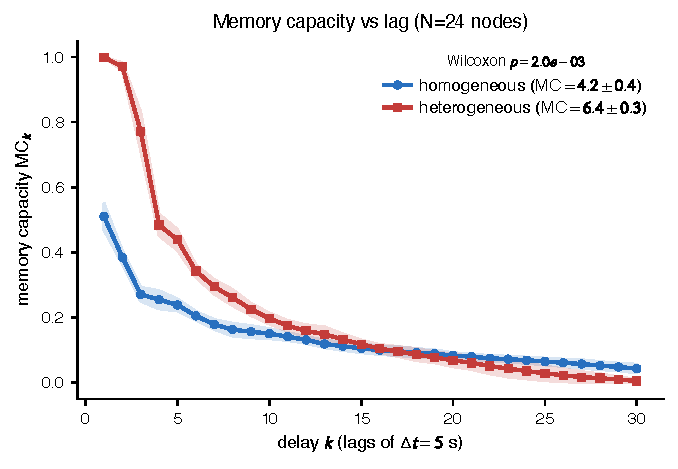
\includegraphics[width=0.66\linewidth]{../figures/chapter5/mc_curve.pdf}
  \caption[Memory capacity versus delay: heterogeneity broadens memory]{Linear memory capacity $\mathrm{MC}_k$ as a function of delay $k$ for a homogeneous bank (all \PEO{} 0.3/0.09 nodes) versus a heterogeneous composition bank ($\tau\approx 3$--$26$\,s). The heterogeneous bank broadens recoverable memory across lags, raising total memory capacity from $4.2$ to $6.4$ (a $1.54\times$ increase; Wilcoxon $p=0.002$ over ten seeds), with the gain concentrated at short-to-intermediate lags. Shaded bands are $\pm 1$\,SD over ten random input/bank seeds. $N=24$ leaky nodes, random uniform input, linear (ridge) read-out; in-silico devices built from the \Cref{ch:comparative} parameter cards.}
  \label{fig:ch5_mc_curve}
\end{figure}

\paragraph{Composition sweep and the single-node optimum.} The same benchmarks, run on single-composition banks, rank the compositions against one another and so test the Demonstration-A claim that one cell suffices for a single-timescale task. \Cref{fig:ch5_composition_sweep} shows that the lead cell \PEO{}~0.3/0.09 attains the highest single-composition memory capacity ($3.98 \pm 0.19$, mean $\pm$ SD over ten seeds), while the neighbouring \PEO{}~0.3/0.045 cell is marginally better on the \NARMA{} system-identification benchmark \cite{AtiyaParlos2000} (NRMSE $0.587 \pm 0.019$ against the lead's $0.616 \pm 0.031$, a close second). Both optima fall in the low-\PEO{} row that \cref{ch:comparative} identifies as carrying the longer fading-memory times, so the benchmark ranking is consistent with the composition result rather than an artefact of the simulation. This supports the Demonstration-A statement: for a single-timescale feature, the lead composition is the memory-capacity optimum and a heterogeneous bank is unnecessary. The \NARMA{} numbers carry only \emph{relative} weight: the absolute error is high ($\approx 0.6$--$0.8$) because a bank of independent, non-recurrent nodes is a weak \NARMA{} reservoir, so the stronger evidence here comes from the capacity measures above (\cref{fig:ch5_mc_curve,fig:ch5_ipc}) and \NARMA{} serves only to corroborate the composition ranking --- a limitation stated rather than hidden, and one a recurrent or delay-feedback architecture would relax.

\begin{figure}[t]
  \centering
  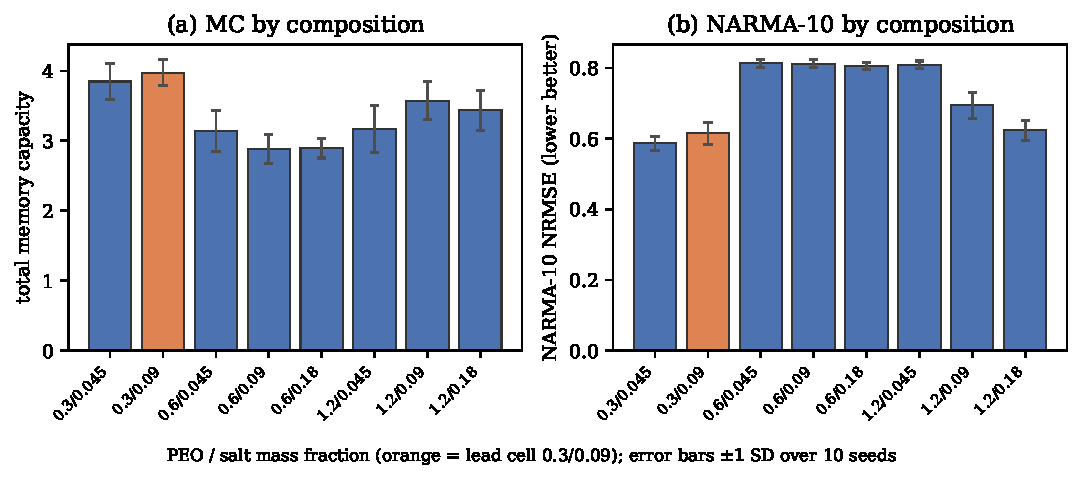
\includegraphics[width=\linewidth]{../figures/chapter5/composition_sweep.pdf}
  \caption[Memory capacity and NARMA across the composition grid]{(a)~Total linear memory capacity and (b)~\NARMA{} reconstruction error (NRMSE, lower is better) for single-composition reservoirs across the \PEO{}/\LiTf{} grid. The lead cell \PEO{}~0.3/0.09 (orange) attains the highest memory capacity; the neighbouring 0.3/0.045 cell is marginally better on \NARMA{}. Both optima fall in the low-\PEO{} row anticipated by \cref{ch:comparative}. Only the \emph{relative} composition ranking is claimed: absolute \NARMA{} NRMSE is high because a bank of independent, non-recurrent leaky nodes is a weak \NARMA{} reservoir.}
  \label{fig:ch5_composition_sweep}
\end{figure}

\paragraph{Linear and nonlinear capacity.} Memory capacity counts only what is \emph{linearly} recoverable. The information-processing-capacity framework of Dambre et al.\ completes the picture by decomposing the total capacity into orthogonal polynomial degrees: degree-one (single-lag) terms give the linear capacity --- essentially the memory capacity --- while degree-two terms (per-lag squares and cross-lag products of the input) give the nonlinear capacity that only a nonlinear reservoir can supply, the whole bounded above by the node count $N$ \cite{Dambre2012}. \Cref{fig:ch5_ipc} reports the split. Even the homogeneous bank carries a substantial nonlinear capacity ($2.7$ of a total $7.1$), which quantitatively supports the interpretation that the compressive potentiation of \cref{ch:comparative} supplies a usable nonlinear response --- the second of the two reservoir prerequisites, alongside fading memory --- rather than merely storing a linear echo. Heterogeneity raises the total capacity from $7.1$ to $11.6$ (paired Wilcoxon $p=0.002$), lifting the linear and nonlinear parts together. The nonlinear capacity is almost entirely degree-two \emph{self} terms (the per-node squaring of the write); cross-lag product terms are negligible, which is the signature of an \emph{independent}, non-recurrent bank that does not multiply inputs across nodes --- consistent with this architecture being, by design, the conservative hard case. That the total sits well below the $N$ bound is likewise expected for leaky nonlinear nodes.

\begin{figure}[t]
  \centering
  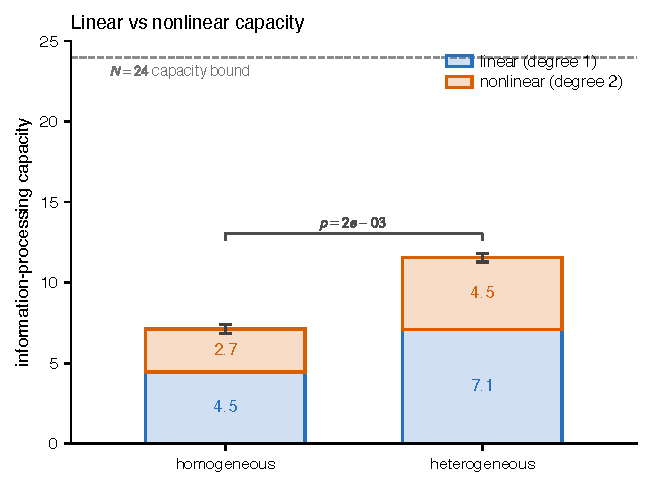
\includegraphics[width=0.52\linewidth]{../figures/chapter5/ipc_capacity.pdf}
  \caption[Information-processing capacity: linear versus nonlinear]{Information-processing capacity \cite{Dambre2012} split into linear (degree-one) and nonlinear (degree-two) parts, for the homogeneous versus the heterogeneous bank ($N=24$, ten seeds). A nonzero nonlinear capacity in both banks indicates that the compressive write supplies a usable nonlinear response, not just linear memory; heterogeneity raises the total from $7.1$ to $11.6$ (paired Wilcoxon $p=0.002$). The dashed line is the $N=24$ upper bound; error bars are $\pm 1$\,SD on the total over seeds.}
  \label{fig:ch5_ipc}
\end{figure}

%% ------------------------------------------------------------
\section{Affective Computing}\label{sec:ch5_affect}
%% ------------------------------------------------------------

Affective computing --- the recognition of human emotional and physiological state by machines --- was framed by Picard as a route to more natural human--computer interaction, classically from \emph{peripheral} physiological signals that are slow, wearable-friendly, and unobtrusive to acquire \cite{Picard1997}. It is the flagship domain of this chapter, for two reasons that follow directly from \cref{ch:comparative}. First, the device timescale window --- fading-memory times from a few seconds to tens of seconds --- sits natively on top of the bands that carry affective information, so no aggressive time-rescaling is needed to bring signal and substrate into register (\cref{tab:ch5_bands}). Second, affective information is \emph{intrinsically multi-timescale}: a fast phasic electrodermal response, a respiration- and heart-rate-variability rhythm of a few seconds, and a tonic level that drifts over minutes all carry state at once~\cite{Boucsein2012EDA,TaskForce1996HRV,ChourpiliadisBhardwaj2022}. That structure is the signal-driven motivation for a heterogeneous bank, and it is also the deployment narrative for an organic, flexible, biocompatible, low-power substrate worn on the skin. \Cref{fig:ch5_tau_coverage} makes the match concrete: it places each composition cell at its measured fading-memory time $\tau$ on the same axis as the affective bands, so that the coverage of the device family --- and, candidly, the one band it does not reach with composition alone --- can be read off directly.

\begin{table}[t]
  \centering
  \small
  \caption[Affective signal timescales and device coverage]{Characteristic timescales of the peripheral affective signals used in this chapter, and the composition cells whose fading-memory window covers them~\cite{Boucsein2012EDA,TaskForce1996HRV,ChourpiliadisBhardwaj2022}. The grid of \cref{ch:comparative} spans the full range, with the lead \PEO{}~0.3 cells serving the slow LF-HRV band.}
  \label{tab:ch5_bands}
  \setlength{\tabcolsep}{5pt}
  \begin{tabular}{lll}
    \toprule
    Affective signal & Timescale & Device coverage \\
    \midrule
    Phasic EDA (SCR) & $\sim$1--10\,s   & low--mid \PEO{} ($t_{1/2}$ 3--19\,s) \\
    Respiration      & $\sim$3--5\,s    & mid \PEO{} \\
    HRV, HF band     & $\sim$2.5--7\,s  & mid \PEO{} \\
    HRV, LF band     & $\sim$7--25\,s   & \PEO{}~0.3 ($\tau \approx 19$--26\,s) \\
    Tonic SCL        & minutes          & slowest / drive-boosted \\
    \bottomrule
  \end{tabular}
\end{table}

\begin{figure}[t]
  \centering
  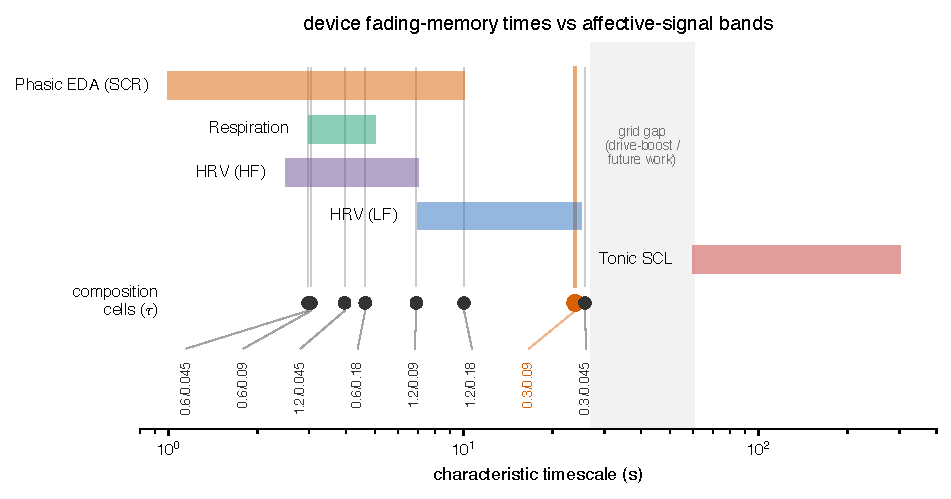
\includegraphics[width=0.82\linewidth]{../figures/chapter5/tau_coverage.pdf}
  \caption[Device timescales versus affective-signal bands]{The \Cref{ch:comparative}-to-\Cref{ch:temporal} bridge as a picture. Each \PEO{}/\LiTf{} composition cell is placed at its measured fading-memory time $\tau$ (markers, lower track) on the same logarithmic time axis as the characteristic timescale bands of the peripheral affective signals (coloured bars; \cref{tab:ch5_bands}). The composition grid ($\tau\approx 3$--$26$\,s) spans the phasic-EDA, respiration and HRV bands, with the lead cell \PEO{}~0.3/0.09 (orange) sitting in the slow LF-HRV band. The tonic, minutes-scale band is not reached by composition alone (shaded gap) and would require the drive-amplitude knob of \cref{ch:comparative} or a slower future cell. This is the visual form of the design rule: an application selects a timescale, and performance follows from how well the device family covers it.}
  \label{fig:ch5_tau_coverage}
\end{figure}

The experiments that follow use the Wearable Stress and Affect Detection corpus (\WESAD{}) of Schmidt et al.\ \cite{Schmidt2018WESAD}: fifteen subjects wearing a chest sensor that records electrodermal activity, respiration, temperature, and an electrocardiogram, with periods labelled baseline, stress, or amusement. \WESAD{} is used in two complementary ways --- as a source of real physiological streams whose multi-lag temporal context the reservoir must encode (\cref{sec:ch5_physio}), and as a downstream affective-classification task (\cref{sec:ch5_wesad}).

%% ------------------------------------------------------------
\section{Physiological Temporal-Context Reconstruction}\label{sec:ch5_physio}
%% ------------------------------------------------------------

The benchmarks of \cref{sec:ch5_benchmarks} prove that a spread of device timescales broadens memory on a \emph{random} input. This section puts that property to a more demanding test on the real, intrinsically multi-timescale affective signals introduced in \cref{sec:ch5_affect}, isolating the multi-timescale \emph{encoding} question before turning to final labels (\cref{sec:ch5_wesad}).

The reservoir is run continuously over each \WESAD{} session at $\Delta t = \SI{1}{\second}$ on four chest channels --- electrodermal activity, respiration, temperature, and an electrocardiogram-derived heart rate --- and a linear read-out reconstructs each channel at delays of $1$, $3$, $8$, $20$ and \SI{45}{\second}. These delays span fast phasic and beat-to-beat context, respiration- and HF-HRV-scale context, and tonic, LF-HRV-scale context~\cite{Boucsein2012EDA,TaskForce1996HRV}. Evaluation is leave-one-subject-out over all fifteen subjects, with $N=48$ nodes per bank.

\Cref{tab:ch5_physio} reports the held-out reconstruction quality. A memoryless bank barely improves on instantaneous input ($R^2 = 0.674$ against $0.673$): with no fading memory, the past is simply not available. Memory of a single timescale lifts $R^2$ to $0.74$, and the heterogeneous composition bank reaches the best single-bank score, $0.756$ --- a gain of $+0.084$ over instantaneous input and $+0.012$ over the best same-size homogeneous control. This last increment is small but unambiguous: scored per subject and paired against the best homogeneous bank across the fifteen subjects, the heterogeneous bank wins in \emph{all fifteen} (Wilcoxon signed-rank $p < 10^{-4}$), so unlike the affective-label increment of \cref{sec:ch5_wesad} it separates cleanly from zero. The mechanism is visible in the band-resolved columns: the fast homogeneous bank is best at the fastest context and the slow homogeneous bank at the slowest, but neither covers the whole vector, whereas the heterogeneous bank is the best \emph{single} bank across the full fast-to-slow physiological context (\cref{fig:ch5_physio}). This is the affect-aligned statement of ``heterogeneity is a computational resource'' on real signals, and it is exactly the result that the final-label classifier of \cref{sec:ch5_wesad} cannot expose.

\begin{table}[t]
  \centering
  \small
  \setlength{\tabcolsep}{5pt}
  \caption[Physiological temporal-context reconstruction on WESAD]{Leave-one-subject-out held-out $R^2$ for multi-lag physiological context reconstruction on \WESAD{} ($N=48$ nodes; means over ten bank seeds where applicable). Bands are reconstruction delays: fast $=1$--$3$\,s, mid $=8$\,s, slow $=20$--$45$\,s. The heterogeneous bank gives the best single-bank score across the full context vector; each homogeneous bank wins only its own band. The heterogeneous advantage over the best homogeneous bank holds in all fifteen subjects (paired Wilcoxon $p<10^{-4}$).}
  \label{tab:ch5_physio}
  \begin{tabular}{lcccc}
    \toprule
    Bank & overall $R^2$ & fast & mid & slow \\
    \midrule
    Instantaneous     & 0.673 & 0.715 & 0.670 & 0.632 \\
    Memoryless        & 0.674 & 0.721 & 0.667 & 0.630 \\
    Homogeneous, fast & 0.741 & \textbf{0.815} & 0.735 & 0.669 \\
    Homogeneous, slow & 0.744 & 0.787 & 0.724 & \textbf{0.711} \\
    Heterogeneous     & \textbf{0.756} & \textbf{0.815} & \textbf{0.737} & 0.708 \\
    \bottomrule
  \end{tabular}
\end{table}

\begin{figure}[t]
  \centering
  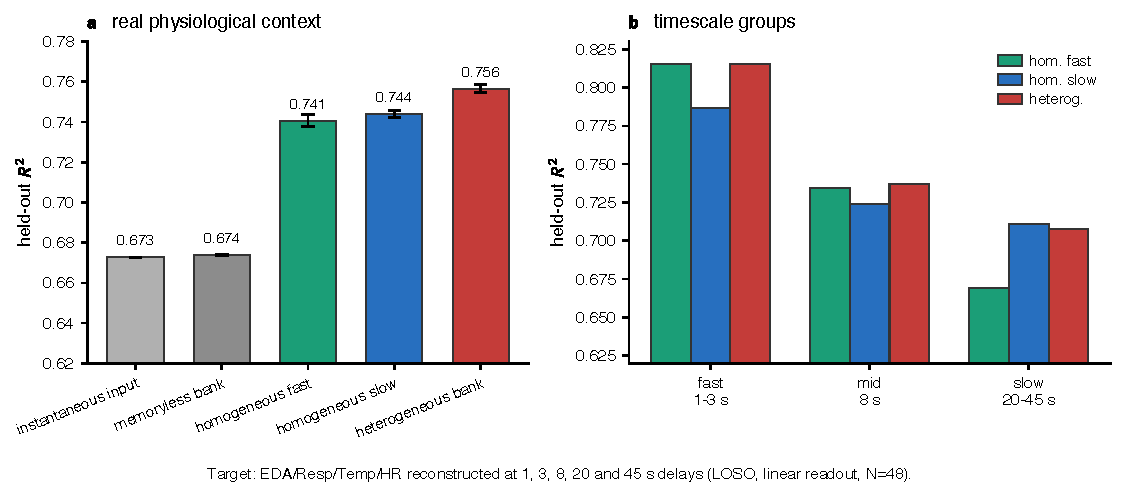
\includegraphics[width=0.82\linewidth]{../figures/chapter5/physio_context_reconstruction.pdf}
  \caption[Physiological temporal-context reconstruction on WESAD]{Multi-lag physiological context reconstruction on real \WESAD{} streams (chest EDA, respiration, temperature, and ECG-derived heart rate). A linear read-out reconstructs each channel at delays of $1$, $3$, $8$, $20$ and $45$\,s from the reservoir state (leave-one-subject-out, $N=48$). The heterogeneous composition bank gives the best single-bank held-out $R^2$ ($0.756$) across the full fast-to-slow context vector, ahead of the best same-size homogeneous control ($0.744$) and well ahead of instantaneous input ($0.673$). Fast and slow homogeneous banks each win only their own band.}
  \label{fig:ch5_physio}
\end{figure}

%% ------------------------------------------------------------
\section{WESAD Affective Classification}\label{sec:ch5_wesad}
%% ------------------------------------------------------------

The downstream task is affective-state classification from the \WESAD{} physiological streams with the device reservoir and a leave-one-subject-out linear read-out. It is reported as a scoped application demonstration: the measured device models support affective classification under the constrained read-out used here, and the contribution of timescale heterogeneity to final labels is reported with error bars, including where it is null. For external calibration, the study that introduced \WESAD{} reports a three-class chest accuracy of $76.5\%$ at macro-F1 $\approx 0.72$ with engineered window features and conventional classifiers under the same leave-one-subject-out protocol, and a binary stress-detection accuracy of $\approx 93\%$ \cite{Schmidt2018WESAD}; the device reservoir's scores below are of the same order. Placed against the wider \WESAD{} literature (\cref{tab:ch5_sota}), which spans engineered-feature classifiers and trained deep networks, the device reservoir's leave-one-subject-out macro-F1 sits in the published performance band, but metric and protocol differences preclude ranking. The comparison shows that a bank of slow organic-memristor models read by a single linear regression can reach a meaningful \WESAD{} performance level under this protocol.

\begin{table}[t]
  \centering
  \small
  \caption[The device reservoir against the WESAD literature]{The device reservoir against representative published \WESAD{} systems. Figures are as reported by each study: classification \emph{accuracy} for the engineered-feature and deep-network systems, the stricter class-balanced \emph{macro-F1} for this work. Metrics and validation protocols differ across studies (Schmidt et al.\ and this work use leave-one-subject-out), so the table is context rather than a head-to-head ranking; its purpose is to show that slow organic-device states with a single linear read-out reach a meaningful WESAD performance level without a trained feature extractor. Binary $=$ stress vs.\ non-stress; three-class $=$ baseline/stress/amusement.}
  \label{tab:ch5_sota}
  \setlength{\tabcolsep}{3pt}
  \begin{tabularx}{\linewidth}{@{}>{\raggedright\arraybackslash}p{2.7cm}>{\raggedright\arraybackslash}Xcc@{}}
    \toprule
    Study & Approach & Three-class & Binary \\
    \midrule
    Schmidt et al.\ (2018)~\cite{Schmidt2018WESAD}   & engineered features, AdaBoost/RF & $76.5\%$ (F1 $0.72$) & $93.0\%$ \\
    Bobade \& Vani (2020)~\cite{Bobade2020}          & engineered features, neural net  & $84.3\%$ & $95.2\%$ \\
    Gil-Mart{\'\i}n et al.\ (2022)~\cite{GilMartin2022} & CNN on spectral features      & $85.1\%$ & $96.6\%$ \\
    \textbf{This work} & device-reservoir states, linear read-out & F1 $0.758$ & F1 $0.894$ \\
    \bottomrule
  \end{tabularx}
\end{table}

\paragraph{Demonstration~A: a single composition suffices for a single-timescale feature.} Binary stress-versus-baseline classification from electrodermal activity, read out at the window level from the lead composition alone, reaches a leave-one-subject-out macro-F1 of $0.894$ (\cref{fig:ch5_wesad}a). This supports the Demonstration-A claim that one well-matched composition can act as a useful affect-aligned node. It comes, however, with an instructive caveat: a static feature baseline (the mean, standard deviation, last value and slope of the same signal) matches it ($0.899$). The 60-second-window task is therefore quasi-static --- the discriminative information sits in the instantaneous signal level, not in its temporal history --- which is exactly why timescale heterogeneity has nothing to contribute here, and why a memory-demanding reformulation is needed to test the heterogeneity claim fairly.

\paragraph{Demonstration~B: streaming three-class tracking.} The fair test is a streaming one: the reservoir runs continuously over each session and the affective class (baseline, stress, or amusement) is read out at \emph{every} step, so that the task is designed to use fading memory rather than a static window summary. \Cref{tab:ch5_wesad} decomposes the result into four matched-size banks. Relative to instantaneous input, adding dimensionality (a same-size memoryless bank) contributes $+0.028$, adding fading memory of a single timescale a further $+0.016$, and adding timescale heterogeneity a final $+0.005$. The measured fading-memory gain over a same-size memoryless bank is a modest but consistent $+0.014$ to $+0.020$. The timescale-heterogeneity increment, however, is $+0.005 \pm 0.011$ --- within seed noise (positive in seven of ten seeds; across sampling intervals from $0.5$ to \SI{4}{\second} the heterogeneous-minus-homogeneous gap stays in $[+0.002,+0.007]$ but never separates from zero). Per class, the best bank reaches F1 $0.90$ on baseline and $0.92$ on stress but only $0.55$ on the amusement class, which is the hard class for every model. The reason is an elicitation limit, not a memory-horizon one: amusement is the shortest \WESAD{} condition (roughly $5.6$\,ks of labelled data against $17.6$\,ks of baseline and $10.0$\,ks of stress) and the lowest in autonomic arousal, so its physiological signature is both weak and under-represented. Consistently, no bank from memoryless to heterogeneous recovers it, which is why the class limits every model rather than discriminating between them.

\begin{table}[t]
  \centering
  \small
  \caption[Streaming three-class affect tracking on WESAD]{Leave-one-subject-out macro-F1 for streaming three-class \WESAD{} tracking (means $\pm$ SD over ten bank seeds; matched input masks). Each increment is the gain over the row above: fading memory contributes a small, consistent gain, while the timescale-heterogeneity increment is within noise (\textit{ns}).}
  \label{tab:ch5_wesad}
  \begin{tabular}{lcc}
    \toprule
    Bank & macro-F1 & increment \\
    \midrule
    Instantaneous (no memory)             & 0.709             & --- \\
    Memoryless (dimensionality only)      & 0.737             & $+0.028$ \\
    Homogeneous (memory, single $\tau$)   & $0.753 \pm 0.009$ & $+0.016$ \\
    Heterogeneous (memory, $\tau$ spread) & $0.758 \pm 0.006$ & $+0.005$ (\textit{ns}) \\
    \bottomrule
  \end{tabular}
\end{table}

\begin{figure}[t]
  \centering
  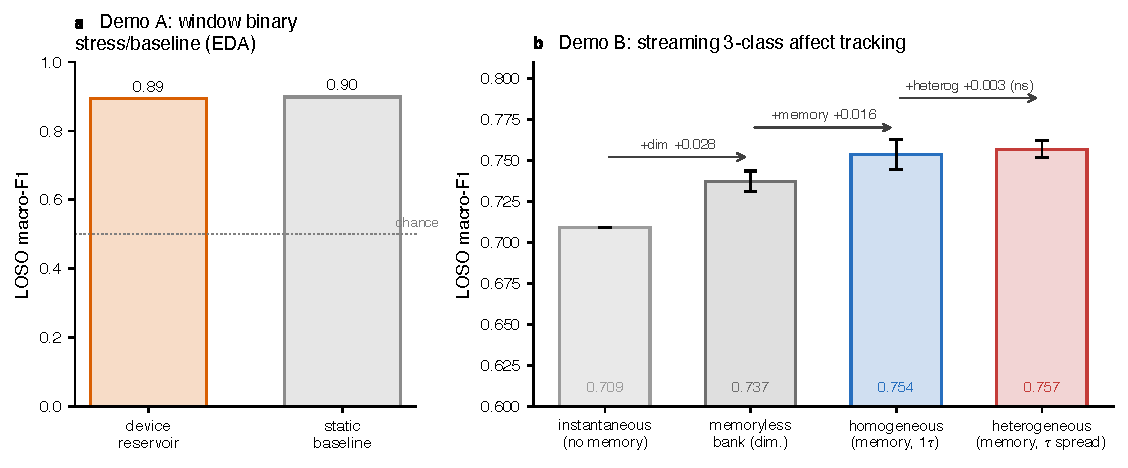
\includegraphics[width=\linewidth]{../figures/chapter5/wesad_affect.pdf}
  \caption[WESAD affective classification with device reservoirs]{Affective classification with in-silico device reservoirs (leave-one-subject-out, linear read-out). (a)~Demonstration A, window-level binary stress-versus-baseline from EDA: the single lead composition matches a static feature baseline, i.e.\ the $60$\,s-window task is quasi-static and requires no fading memory. (b)~Demonstration B, streaming three-class affect tracking (baseline/stress/amusement) decomposed as instantaneous $\rightarrow$ $+$dimensionality $\rightarrow$ $+$fading memory $\rightarrow$ $+$timescale heterogeneity. Fading memory contributes a small but consistent gain; the timescale-heterogeneity increment ($+0.005\pm0.011$) is within seed noise. Error bars are $\pm 1$\,SD over $10$ bank seeds.}
  \label{fig:ch5_wesad}
\end{figure}

\paragraph{Why heterogeneity does not pay off on the labels.} The null is not a failure of the devices but a property of the task. Affect labels are slowly varying, sustained states; their discriminative memory demand is dominated by a single slow, tonic band that the lead composition's relaxation time ($\tau \approx 19$--$26$\,s) already serves. Timescale heterogeneity converts into task performance only when the target requires memory at many distinct lags \emph{simultaneously} --- which the memory-capacity benchmark (\cref{fig:ch5_mc_curve}) and the physiological-context reconstruction (\cref{tab:ch5_physio}) both demand, and on which heterogeneity does pay, but which a single sustained label set does not. The reading carried into \cref{sec:ch5_designrules} is that the measured device models support affective classification under this protocol, that fading memory helps, and that composition-timescale \emph{matching} is the operative design lever --- with heterogeneity a generality and robustness hedge rather than a guaranteed win on any one label set.

%% ------------------------------------------------------------
\section{Continuous Monitoring Under Deployment Conditions}\label{sec:ch5_robust}
%% ------------------------------------------------------------

The scores of \cref{sec:ch5_wesad} are dominated by long stretches of sustained state, where the instantaneous signal level already carries the label --- which is precisely why a static feature baseline ties the reservoir on the quasi-static window task. A wearable in the field is judged on what those averages hide. It must keep working while the wearer moves and the sensor is noisy, and motion artefact is the dominant failure mode of wrist-worn electrodermal and photoplethysmographic sensing. This is a temporal problem on which fading memory has a structural advantage: a leaky integrator is a temporal low-pass that averages transient artefact away, whereas an instantaneous read reacts to every spike.

\Cref{fig:ch5_robust_monitoring} makes the point on a continuous binary stress detector --- stress versus baseline-plus-amusement, read out at every step, leave-one-subject-out, with the same single linear read-out used throughout. On clean streams every bank is competitive (macro-F1 $\approx 0.91$--$0.92$, of the order of the $\approx 93\%$ binary benchmark of the corpus~\cite{Schmidt2018WESAD}), the static read among them, exactly as the window task warned. As progressively stronger sensor noise and motion-artefact bursts are injected, the instantaneous and memoryless controls degrade steeply --- macro-F1 from $0.914$ to $0.840$ by an injected noise of $\sigma = 0.4$ of the signal range --- while the fading-memory banks barely move, holding $\approx 0.92$ across the whole range. At $\sigma = 0.4$ the advantage of the heterogeneous memory bank over the instantaneous read is $+0.088$, positive in all fifteen subjects (paired Wilcoxon $p < 10^{-4}$); and even on clean streams, fading memory roughly halves the false-alarm rate ($0.046 \to 0.026$), the spurious-alert cost that most limits a deployed affect monitor. The active ingredient is memory itself, not its spread: the homogeneous and heterogeneous banks are equally robust, consistent with the design rule below. Two boundaries are reported with the result rather than around it: the accuracy gain in the narrow window straddling label transitions is positive ($0.747 \to 0.775$) but not resolved across subjects, and the detection latency is comparable across banks, set by the prediction-smoothing horizon rather than by the device. The deployment-relevant statement is therefore specifically about robustness --- under the corruption a real wearable faces, the temporal device sustains a stress detector that the static baseline, competitive only in laboratory-clean conditions, does not.

\begin{figure}[t]
  \centering
  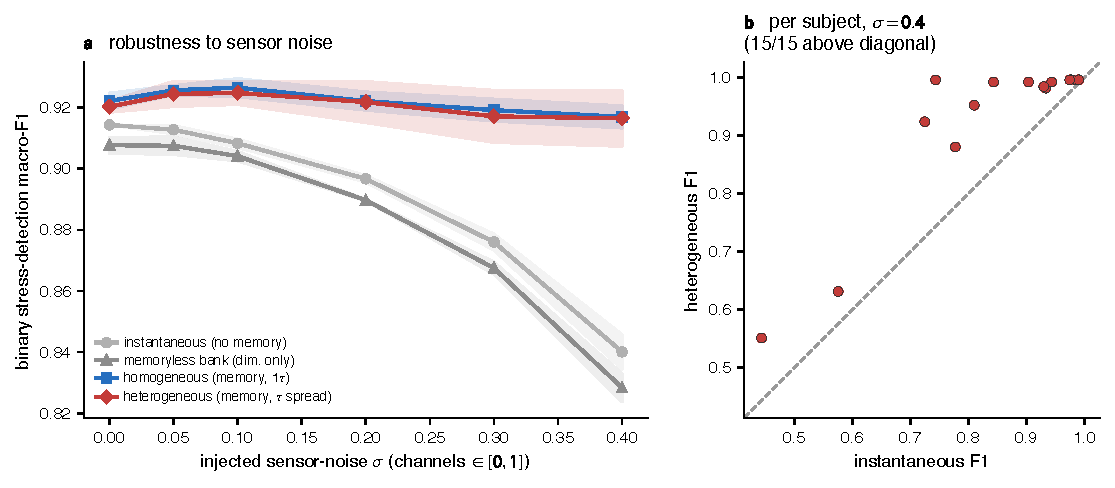
\includegraphics[width=\linewidth]{../figures/chapter5/robust_monitoring.pdf}
  \caption[Continuous stress monitoring is robust to sensor noise]{Continuous stress monitoring with device reservoirs (binary stress vs.\ baseline-plus-amusement, per-step, leave-one-subject-out, linear read-out). (a)~Detection macro-F1 against the magnitude $\sigma$ of injected sensor noise and motion-artefact bursts: the fading-memory banks (homogeneous, heterogeneous) stay flat at $\approx 0.92$, while the instantaneous and memoryless controls collapse, because temporal integration rejects transient artefact. Bands are $\pm 1$\,SD over seeds. (b)~Per-subject scores at $\sigma=0.4$: the heterogeneous memory bank beats the instantaneous read in all fifteen subjects (paired Wilcoxon $p<10^{-4}$). Memory, not its heterogeneity, is the active ingredient; the homogeneous bank is equally robust.}
  \label{fig:ch5_robust_monitoring}
\end{figure}

\paragraph{Cross-corpus replication.} A single corpus cannot establish generality, so the robustness test was repeated on an independent dataset: the PhysioNet Non-EEG corpus of Birjandtalab et al.~\cite{Birjandtalab2016}, twenty subjects wearing a \emph{different} wrist sensor (an Affectiva Q recording electrodermal activity and skin temperature, with a pulse-oximeter heart rate) through relaxation and cognitive, emotional, and physical stress phases. Taking cognitive and emotional stress as the stress class against relaxation --- the psychosocial analogue of the \WESAD{} stressor, with the physical-exertion phase held out as a different mechanism whose racing heart rate is trivially separable from the instantaneous signal alone --- and running the identical detector reproduces the \WESAD{} result on this independent sensor and population (\cref{tab:ch5_crosscorpus}). The corpus is harder in absolute terms (clean macro-F1 $\approx 0.65$--$0.68$, against $\approx 0.91$ on the cleaner \WESAD{} chest signals) and, as on \WESAD{}, the clean-stream memory advantage is small and not resolved. But under sensor noise the same divergence reappears, more sharply: the instantaneous detector falls from $0.651$ to $0.516$ while the fading-memory bank holds near $0.66$, a $+0.130$ advantage at $\sigma=0.4$ that is positive in nineteen of the twenty subjects (paired Wilcoxon $p<10^{-5}$). The noise-robustness of the temporal substrate is therefore not a property of one dataset; it transfers to a new corpus, sensor, and population.

\begin{table}[t]
  \centering
  \small
  \caption[Cross-corpus replication on the PhysioNet Non-EEG dataset]{Cross-corpus replication of the noise-robustness result on the independent PhysioNet Non-EEG stress corpus~\cite{Birjandtalab2016} (twenty subjects; Affectiva Q wrist electrodermal activity and temperature plus pulse-oximeter heart rate; cognitive and emotional stress versus relaxation; leave-one-subject-out, linear read-out). As on \WESAD{}, the instantaneous detector collapses under injected sensor noise while the fading-memory banks hold; the heterogeneous-minus-instantaneous advantage at $\sigma=0.4$ is $+0.130$ ($19/20$ subjects, $p<10^{-5}$). Memory, not its spread, is again the active ingredient.}
  \label{tab:ch5_crosscorpus}
  \setlength{\tabcolsep}{8pt}
  \begin{tabular}{lcc}
    \toprule
    Detector & macro-F1 (clean) & macro-F1 ($\sigma=0.4$) \\
    \midrule
    Instantaneous (no memory) & 0.651 & 0.516 \\
    Homogeneous (memory)      & \textbf{0.682} & \textbf{0.657} \\
    Heterogeneous (memory)    & 0.667 & 0.646 \\
    \bottomrule
  \end{tabular}
\end{table}

%% ------------------------------------------------------------
\section{Toward a Worn Device: Sensor Site and Operating Budget}\label{sec:ch5_deploy}
%% ------------------------------------------------------------

The robustness of the previous section is a laboratory statement until two further questions are answered: whether the advantage survives a consumer-grade sensor, and what the device would cost to run. Both are answered from the same measured ingredients --- the \WESAD{} wrist recordings and the device constants of \cref{ch:poc} --- without any new assumption.

\paragraph{Sensor site.} \WESAD{} records every session twice: from a chest strap (the clean electrocardiogram and respiration used so far) and from an Empatica E4 wrist band, the form factor of a real affective wearable but with fewer and far noisier channels --- skin conductance, skin temperature, and a photoplethysmogram from which heart rate must be recovered, with no respiration. Re-running the continuous stress detector of \cref{sec:ch5_robust} on the wrist signals (\cref{tab:ch5_wrist}) tells a consistent story. The static, instantaneous detector loses ground on the wrist, its clean macro-F1 falling from $0.914$ on the chest to $0.881$ as the noisier photoplethysmographic heart rate and the missing respiration channel degrade the instantaneous signal. The fading-memory reservoir is essentially unaffected by the move to the wrist ($0.920 \to 0.922$): it recovers from temporal context what the static read loses to channel quality. The memory advantage is therefore much larger on the consumer wrist than on the chest ($+0.041$ on clean streams against $+0.006$, and a sustained $+0.069$ under injected noise), which is the right way round for deployment --- the harder, more realistic sensor is exactly where the temporal substrate helps most, and fading memory cuts the wrist false-alarm rate by about a third ($0.062 \to 0.040$).

\begin{table}[t]
  \centering
  \small
  \caption[Stress detection: chest versus consumer wrist sensor]{Continuous binary stress-detection macro-F1 on the \WESAD{} chest strap versus the Empatica E4 wrist band (leave-one-subject-out, linear read-out). Moving to the noisier consumer sensor degrades the instantaneous (static) detector but not the fading-memory reservoir, so the memory advantage is larger on the wrist; $\sigma$ is the injected sensor-noise level of \cref{fig:ch5_robust_monitoring}.}
  \label{tab:ch5_wrist}
  \setlength{\tabcolsep}{5pt}
  \begin{tabularx}{\linewidth}{@{}>{\raggedright\arraybackslash}Xcccc@{}}
    \toprule
    & \multicolumn{2}{c}{Chest} & \multicolumn{2}{c}{Wrist E4} \\
    \cmidrule(lr){2-3}\cmidrule(lr){4-5}
    Detector & clean & $\sigma=0.4$ & clean & $\sigma=0.4$ \\
    \midrule
    Instantaneous (no memory)   & 0.914 & 0.840 & 0.881 & 0.847 \\
    Memory reservoir (het)      & \textbf{0.920} & \textbf{0.916} & \textbf{0.922} & \textbf{0.916} \\
    \bottomrule
  \end{tabularx}
\end{table}

\paragraph{Operating budget.} The reservoir's appeal for a worn device is that temporal filtering is delegated to the material dynamics: the dynamics are fixed and untrained, and only the linear read-out is fitted, by a single closed-form ridge solve rather than gradient descent. The trained part is therefore one $(N{+}1)\times K$ weight matrix --- $75$ weights for the $N=24$, three-class banks here, $147$ for the $N=48$ banks --- against the $10^{4}$ to $10^{6}$ trainable weights of the deep models usually brought to wearable affect, a reduction of roughly two to four orders of magnitude that puts on-device, per-user calibration within reach. The energy budget follows from the measured device of \cref{ch:poc}: at the proof-of-concept energy of $\approx\SI{50}{\nano\joule}$ per write event ($\approx\SI{6}{\femto\joule\per\micro\metre\squared}$ over the \SI{0.0825}{\square\centi\metre} junction), charging each of $N$ nodes once per one-second update draws of order a microwatt ($\approx\SI{1.2}{\micro\watt}$ at $N=24$), while the read-out is $N\,K$ multiply--accumulates, well under a nanojoule per step. These are unoptimised, large-area figures; reducing the junction toward the integrated-device regime would cut the per-event energy by orders of magnitude. The point is the order of magnitude and the contrast in kind: the device responds in the sub-kilohertz regime, comfortably above the sub-hertz bandwidth of affective physiology, so the substrate is never the bottleneck, and the temporal feature extraction that a digital pipeline would compute explicitly is performed by the device dynamics during the write/read cycle. The full budget and its assumptions are tabulated in \siTempRef{app:ch5_deploy}.

%% ------------------------------------------------------------
\section{Design Rule: Match Timescale to Task}\label{sec:ch5_designrules}
%% ------------------------------------------------------------

\Cref{sec:ch5_benchmarks,sec:ch5_physio,sec:ch5_wesad} complete the design rule opened in \cref{ch:comparative}. Composition and drive \emph{set} the fading-memory timescale; an application \emph{selects} one timescale, or a set of timescales, and performance follows from how well the device family covers them (\cref{fig:ch5_tau_coverage}). The composition sweep gives the single-timescale case (\cref{fig:ch5_composition_sweep}): the lead cell is the memory-capacity optimum because its relaxation time best matches a seconds-scale target. The multi-lag physiological task gives the opposite case (\cref{tab:ch5_physio}): when the target spans bands that no single cell covers, the bank whose timescales are \emph{spread} to match them is the best single choice.

\paragraph{Memory first, heterogeneity as a generality hedge.} The results give a consistent account of what these resources are worth, drawn together in \cref{tab:ch5_summary}. The first-order effect is \emph{fading memory itself}: every memory bank, homogeneous or heterogeneous, far exceeds the memoryless and instantaneous baselines, and the gap widens to as much as $+0.08$ macro-F1 under the sensor noise of a worn device (\cref{sec:ch5_robust,sec:ch5_deploy}). The second-order effect is the \emph{spread} of timescales. Where the task demands memory at many lags at once --- random-input memory capacity (a $1.54\times$ broadening, $p=0.002$; \cref{fig:ch5_mc_curve}) and real-physiology context reconstruction ($+0.012$ in held-out $R^2$ over the best homogeneous bank, $15/15$ subjects, $p<10^{-4}$; \cref{tab:ch5_physio}) --- heterogeneity is a measurable, statistically resolved resource. Where a single slow timescale already dominates, as in the sustained stress labels and the single-channel monitoring task, the best-matched single composition is as good or marginally better, exactly as Demonstration~A anticipated. The two readings combine into a deployment rule: because a heterogeneous bank gives up at most about a hundredth of a point on the single-timescale tasks but gains substantially on the multi-timescale ones, it is the rational default for a substrate fabricated once and reused across an unknown mix of affective tasks. Crucially for the materials argument of this thesis, that heterogeneity is \emph{low-cost and intrinsic}: it arises naturally in a solution-processed device family through composition spread, device-to-device scatter, and --- as further, illustrative knobs catalogued in \cref{ch:comparative} but not required by the quantitative banks here --- electrolyte chemistry and drive amplitude.

\begin{table}[t]
  \centering
  \small
  \caption[Fading memory versus its spread across the affective workload]{Fading memory versus its spread across the affective workload of this chapter. Every memory bank (homogeneous, heterogeneous) far exceeds the memoryless instantaneous baseline --- decisively so under the sensor noise of a worn device --- so fading memory is the first-order resource. The heterogeneous bank then wins where several timescales matter at once (physiological context), while the best-matched single composition wins where one timescale dominates (sustained labels, single-channel monitoring); the gap between them never exceeds about $0.01$ macro-F1. Bold marks the best bank per row. Scores from \cref{tab:ch5_physio,tab:ch5_wesad} and \cref{sec:ch5_robust,sec:ch5_deploy}.}
  \label{tab:ch5_summary}
  \setlength{\tabcolsep}{4pt}
  \begin{tabularx}{\linewidth}{@{}>{\raggedright\arraybackslash}Xlccc@{}}
    \toprule
    Affective task & Metric & Instantaneous & Homogeneous & Heterogeneous \\
    \midrule
    Physiological context (multi-$\tau$) & $R^2$       & 0.673 & 0.744 & \textbf{0.756} \\
    Three-class affect tracking          & macro-F1    & 0.709 & 0.753 & \textbf{0.758} \\
    Stress monitoring, clean             & macro-F1    & 0.914 & \textbf{0.922} & 0.920 \\
    Stress monitoring, $\sigma{=}0.4$    & macro-F1    & 0.840 & \textbf{0.917} & 0.916 \\
    Wrist stress, clean                  & macro-F1    & 0.881 & \textbf{0.930} & 0.922 \\
    Wrist stress, $\sigma{=}0.4$         & macro-F1    & 0.847 & \textbf{0.918} & 0.916 \\
    \bottomrule
  \end{tabularx}
\end{table}

\paragraph{Operating point and integration.} The same parameter cards that drive the simulations also fix the deployment envelope. The devices operate in the sub-kilohertz regime in which affective physiology lives, so the slow response that disqualifies them for fast logic is exactly what suits them to on-skin sensing. The read-out is assumed sub-threshold and state-preserving, which sets a read-voltage and read-disturb budget that any circuit implementation must respect; and the device-to-device scatter that a memory application would treat as a yield problem is, in the reservoir setting, part of the computational substrate. \Cref{fig:ch5_robustness} makes this last point quantitative and is perhaps the clearest single statement of the reservoir's tolerance to the imperfection of solution processing: total memory capacity is reported against the magnitude of injected device-to-device scatter, and the heterogeneous bank holds its advantage across the whole realistic range --- including at the \emph{measured} scatter, \(\sigma(\ln\tau)\approx\num{0.85}\), estimated from the silver \PEO{}/\LiTf{} devices within each fixed composition cell and confirmed to be unexplained by spin speed, anneal, film thickness, or device age (\siTempRef{app:ch5_scatter}). The limiting case is instructive --- a bank of \emph{identical} nodes (zero scatter) is nearly memory-less, because perfectly matched nodes are redundant, so the scatter that yield engineering fights to remove is precisely what a homogeneous reservoir lives on, while the heterogeneous bank additionally carries intrinsic timescale spread and therefore degrades most gracefully. These are the design rules that \cref{ch:comparative} makes available and that an eventual hardware reservoir would inherit.

\begin{figure}[t]
  \centering
  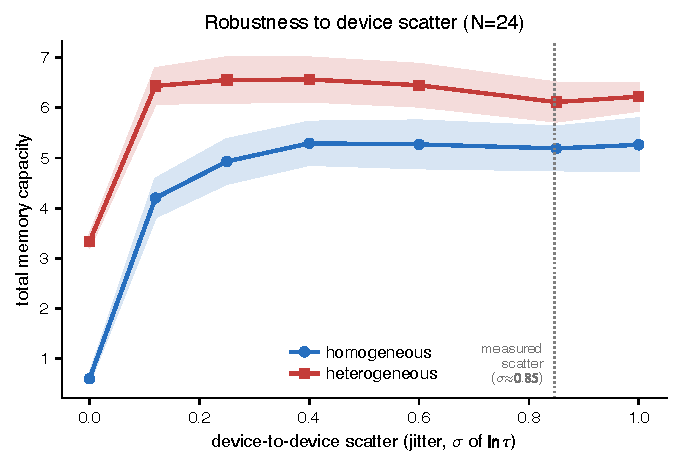
\includegraphics[width=0.6\linewidth]{../figures/chapter5/robustness.pdf}
  \caption[Robustness to device-to-device scatter]{Total memory capacity versus the magnitude of injected device-to-device scatter (jitter on $\tau$, $\beta$ and $\alpha$), for the homogeneous and heterogeneous banks ($N=24$, ten seeds; shaded bands $\pm 1$\,SD). The heterogeneous bank keeps its advantage across the entire realistic spread, including at the measured device-to-device scatter (dotted line: \(\sigma(\ln\tau)\approx\num{0.85}\), derived in \siTempRef{app:ch5_scatter}). A bank of perfectly identical nodes (zero scatter) is nearly memory-less because matched nodes are redundant: the scatter that yield engineering fights to remove is what the reservoir computes on.}
  \label{fig:ch5_robustness}
\end{figure}

%% ------------------------------------------------------------
\section{Limitations and Scope Conditions}\label{sec:ch5_limitations}
%% ------------------------------------------------------------

The claims of this chapter are bounded by scope conditions that are stated here in full, in keeping with the claim discipline of \cref{ch:comparative}.

\paragraph{In silico.} The demonstrations are simulations. Each node is the measured $\phi \otimes \lambda \otimes f$ behavioural model of \cref{sec:ch5_model}, not a bench reservoir, and every figure caption names the data behind it; the step from a fitted per-device model to a wired hardware reservoir is left to future work.

\paragraph{The composition assumption.} As detailed in \cref{sec:ch5_model}, the write nonlinearity and the fading-memory law were measured separately, at different write amplitudes and a single inter-pulse cadence. Composing them assumes the two regimes are compatible and probably under-estimates the coupling between drive and retention. A single matched-amplitude experiment that sweeps pulse count and inter-pulse interval together would remove the assumption; it is the most important bench experiment this chapter calls for.

\paragraph{Operating regime and read-out.} The model is identified, and valid, only in the slow, sub-kilohertz regime of the measurements; affective signals fall natively in this band, but fast temporal tasks are out of scope. Every read-out is a single ridge regression --- a deliberate constraint, since a nonlinear read-out could solve the tasks by itself and would invalidate the reservoir claim --- and the read is assumed sub-threshold and state-preserving.

\paragraph{Heterogeneity axes.} The quantitative heterogeneous banks span the replicated \PEO{}/\LiTf{} composition grid. The chemistry and drive-amplitude axes of \cref{ch:comparative}, being sample-limited ($n\le 2$ per matched cell), enter only as illustrative additional knobs; Demonstration~B is therefore a principle demonstration of composition heterogeneity, not a powered comparison across chemistries. The composition cells that define these banks index \emph{composition}, not film thickness: although spin-coating speed and residual film thickness covary with the \PEO{} fraction, the parameter cards inherited here were shown to be governed by composition rather than thickness (\cref{fig:ch4_thickness_control}, \cref{sec:ch4_materials}), so the heterogeneity exploited in this chapter is compositional in origin.

\paragraph{Corpora, and a reported null.} The affective classification results rest principally on one corpus (\WESAD{}); the deployment-critical noise-robustness finding is replicated on a second, independent corpus, wrist sensor, and population (the PhysioNet Non-EEG dataset, \cref{sec:ch5_robust}), but a broader multi-corpus study, and the affective dimensions beyond stress such as continuous valence and arousal, remain future work. The central negative result --- that timescale heterogeneity does not separably improve final-label classification --- is reported with error bars across seeds and sampling intervals rather than omitted, because it is informative: it localises exactly where heterogeneity helps and where it does not.

%% ------------------------------------------------------------
\section{Summary and Bridge to the Conclusions}\label{sec:ch5_conclusions}
%% ------------------------------------------------------------

This chapter has shown that compact behavioural models of solution-processed polymer-electrolyte memristors, characterised through the three common measurements of \cref{ch:comparative} and read out by a single linear regression, can support temporal-computing demonstrations within the stated in-silico scope. The models produce a resolved memory-capacity gain for heterogeneous banks, give a relative \NARMA{} composition ranking, encode the multi-lag temporal context of real physiological signals, and classify affective state from the \WESAD{} corpus at a leave-one-subject-out macro-F1 of $0.894$ on a binary stress task and $0.758$ on a three-class streaming task. Beyond accuracy on curated splits, the same models sustain a continuous stress detector under the sensor noise and on the consumer wrist band that a worn device must tolerate --- where fading memory holds detection near $0.92$ macro-F1 while a static baseline collapses to $0.84$ ($+0.088$, all fifteen subjects, $p<10^{-4}$) --- at an estimated always-on budget of order a microwatt and only the tens-to-a-hundred trained read-out weights of one ridge solve, against the $10^4$--$10^6$ gradient-trained weights of a deep model of comparable accuracy.

The results resolve into a single design rule that unifies the two experimental chapters. \Cref{ch:comparative} establishes that composition and drive set the device timescale; this chapter establishes that the application selects the timescale, that fading memory is the active computational ingredient, and that a spread of timescales is a measurable resource for memory breadth --- a $1.54\times$ broadening of memory capacity and a consistent gain in physiological-context encoding, both statistically resolved --- even though it is not required when a single slow timescale already dominates a task. The heterogeneity that \cref{ch:comparative} catalogued as a tuning landscape is, in this light, what the computation is built from.

The concluding chapter draws together the contributions of the thesis and its limitations. The most consequential next steps follow directly from the scope conditions above: the matched-amplitude, varied-cadence pulse-train experiment that would convert the composition assumption into measured fact; a powered study of the chemistry and drive-amplitude heterogeneity axes; and a hardware reservoir that replaces the in-silico bank with wired devices, closing the gap between a fitted device model and a physical temporal computer.


%% ---- Standalone close (skipped when \include'd from thesis.tex) ----
%% A unified bibliography is printed from thesis.tex in the thesis build,
%% so the per-chapter \printbibliography runs only in standalone mode.
\ifdefined\thesismode
  \let\thesisstandaloneclose\relax
\else
  \printbibliography[heading=bibintoc, title={References}]
  \def\thesisstandaloneclose{\end{document}}
\fi
\thesisstandaloneclose
